\documentclass[11pt]{article}

\usepackage[a4paper,margin=1in]{geometry}
\usepackage[T1]{fontenc}
\usepackage[utf8]{inputenc}
\usepackage{lmodern}
\usepackage{graphicx}
\usepackage{hyperref}

\hypersetup{
  colorlinks=true,
  linkcolor=black,
  urlcolor=blue,
  pdftitle={LLM Reasoning Telemetry Demo},
  pdfauthor={OpenAI Codex},
  pdfsubject={Stability Oracle demo paper}
}
\setcounter{secnumdepth}{3}
\setcounter{tocdepth}{2}

\title{LLM Reasoning Telemetry Demo\\Project Paper}
\author{Stability Oracle Demo Update}
\date{March 25, 2026}

\begin{document}
\maketitle
\tableofcontents
\newpage

\section{Purpose}

This paper records the first non-HAOS demonstration domain for Stability Oracle:
stepwise LLM reasoning traces.

The purpose is narrow.

\begin{quote}
This demo shows that the oracle can detect structural reasoning drift using only trajectory geometry.
\end{quote}

This is not a cognition model, truth model, or physics experiment.
It is a structural telemetry classification demo.

\section{Frozen Demo Contract}

Demo v1 is intentionally frozen.
The current contract is:

\begin{itemize}
\item telemetry dimension = 8
\item dataset size = 12 traces
\item expected bands: coherent $\rightarrow$ stable, drifted $\rightarrow$ marginal, broken $\rightarrow$ unstable
\item no stochastic components
\item oracle kernel untouched
\end{itemize}

This prevents silent drift while the demo is still serving as the first public proof surface.

\section{Telemetry Definition}

Each reasoning step becomes one telemetry frame with a fixed 8-dimensional vector:

\begin{enumerate}
\item step length norm
\item confidence proxy
\item novelty vs previous step
\item self overlap
\item contradiction score
\item numeric consistency score
\item tool dependency score
\item terminality score
\end{enumerate}

All values are deterministic and bounded to the interval $[0,1]$.
Missing signals are filled conservatively with $0.0$.

\section{Adapter Behavior}

The LLM reasoning adapter uses simple deterministic heuristics:

\begin{itemize}
\item token-count normalization for step length
\item lexical continuity for overlap and novelty
\item explicit correction terms for contradiction detection
\item numeric token persistence for consistency
\item keyword checks for tool dependency
\item final-step markers for terminality
\end{itemize}

The adapter does not call external APIs and does not depend on model internals.

\section{Oracle Integration}

The demo does not modify the oracle kernel.
Instead it performs a narrow wrapper transformation:

\begin{verbatim}
reasoning trace
-> telemetry vectors
-> canonical reasoning state
-> observed transition state
-> OracleEngine.evaluate_transition(...)
\end{verbatim}

This keeps the existing logical oracle as the execution kernel while allowing a foreign trajectory domain to enter through a deterministic surface.

\section{Dataset}

The demo dataset contains twelve traces:

\begin{itemize}
\item 4 coherent traces with correct outcomes
\item 4 drifted traces with incorrect outcomes
\item 4 broken traces with broken outcomes
\end{itemize}

The tasks mix simple arithmetic and simple logical inference.
The goal is not coverage.
The goal is a small, inspectable proof of separation.

\section{Observed Results}

The current demo run produces the following band separation:

\begin{itemize}
\item coherent traces $\rightarrow$ 4 stable
\item drifted traces $\rightarrow$ 4 marginal
\item broken traces $\rightarrow$ 4 unstable
\end{itemize}

The exported CSV and plot are deterministic artifacts.

\begin{figure}[h]
  \centering
  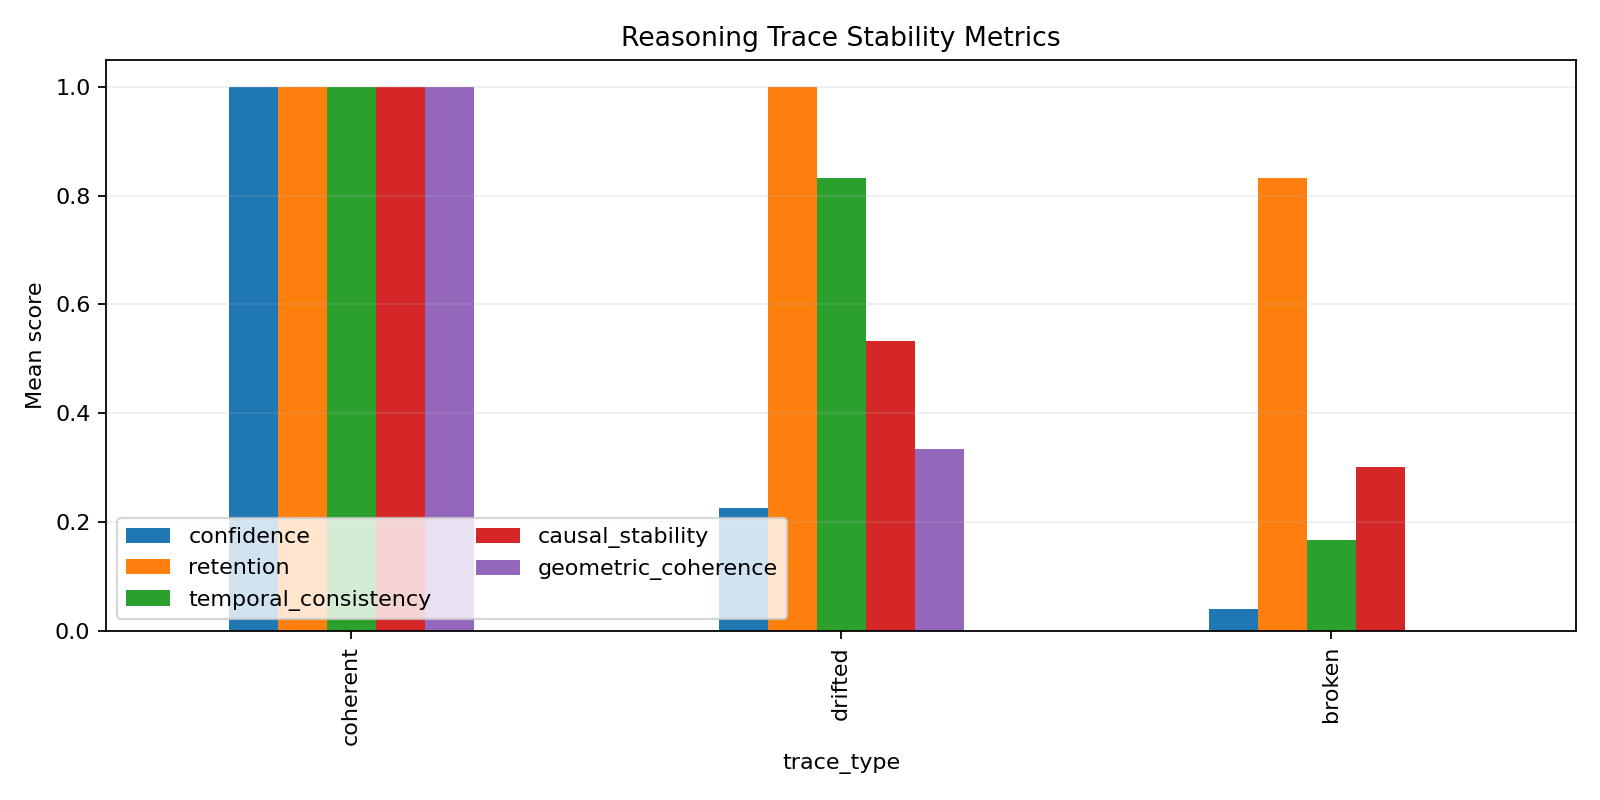
\includegraphics[width=\textwidth]{../../stability_oracle_demo/output/metrics_plot.png}
  \caption{Mean metric scores across coherent, drifted, and broken reasoning traces.}
\end{figure}

\section{Interpretability Artifact}

The demo now exports a second machine-readable artifact:

\begin{verbatim}
trace_explanations.json
\end{verbatim}

For each task it stores:

\begin{itemize}
\item dominant metric contribution
\item transition magnitude
\item recovery score trend
\item final class reason
\end{itemize}

This is useful because the demo is more credible when the label can be explained by a short deterministic rationale instead of a black-box verdict.

\section{Falsification Trace}

The demo also includes one deliberate edge case:
a noisy reasoning trace that deviates in the middle but returns close to its starting line of reasoning.

This trace is currently classified as \texttt{marginal}.
That is the intended result for v1.

It shows that the oracle can tolerate noise without treating every temporary wobble as a structural collapse.

\section{What This Demo Does Not Claim}

This demo does not claim:

\begin{itemize}
\item truth tracking
\item cognition modeling
\item reasoning correctness guarantees
\item model introspection
\item intelligence measurement
\end{itemize}

It only demonstrates that a deterministic geometry-based oracle can classify the structural quality of stepwise traces.

\section{Operational Outputs}

The current demo generates:

\begin{itemize}
\item \texttt{results.csv}
\item \texttt{trace\_explanations.json}
\item \texttt{metrics\_plot.png}
\item a deterministic regression test for band separation
\item a deterministic falsification test for the noisy-return edge trace
\end{itemize}

\section{Conclusion}

This is the right scale for the next milestone.

The demo is:

\begin{itemize}
\item small
\item deterministic
\item reproducible
\item domain-agnostic in method
\item explicit about what it does and does not test
\end{itemize}

Most importantly, it makes the oracle feel like a usable instrument rather than just an architectural claim.

\end{document}
